%! Author = itgramic
%! Date = 05.12.23

% Preamble
\begin{flushleft}
    \subsubsection{pg\_auto\_failover}
    pg\_auto\_failover ist eine PostgreSQL-Erweiterung, die von der Microsoft Subunternehmen Citus Data entwickelt wird.
\end{flushleft}
\begin{flushleft}
    \paragraph{Core-Features}
    Die wichtigsten Features von pg\_auto\_failover sind:
    \begin{itemize}
        \item API
        \item PostgreSQL Extension, also reines PostgreSQL
        \item State Machine Driven
        \item Replikations-Quorum
        \item Citus kompatibel
        \item Azure VM Support
    \end{itemize}
\end{flushleft}
\begin{flushleft}
    \paragraph{Replikation}
    pg\_auto\_failover bietet die Standard PostgreSQL-Replikationen.
\end{flushleft}
\begin{flushleft}
    \paragraph{Proxy}
    pg\_auto\_failover benötigt einen \Gls{HAProxy}, um Load Balancing betreiben zu können\cite{VYXTI7BS}.
\end{flushleft}
\begin{flushleft}
    \paragraph{API / Skripte}
    pg\_auto\_failover bietet ein eigenes CLI-Tool, \texttt{pg\_autoctl}.
    Dieses stellt Commands für das Einbinden neuer Nodes,\\
    das Managen von Nodes (Maintenance resp. Switchover),\\
    Konfigurieren oder Monitoren des Systems zur Verfügung\cite{4X2AKDB6}.
\end{flushleft}
\begin{flushleft}
    \paragraph{Architektur}
    Die Dokumentation resp. Grafik von pg\_auto\_failover \cite{PZZIZ5RT} zeigt auf, wie der Failover funktioniert:
    \begin{figure}[H]
        \centering
        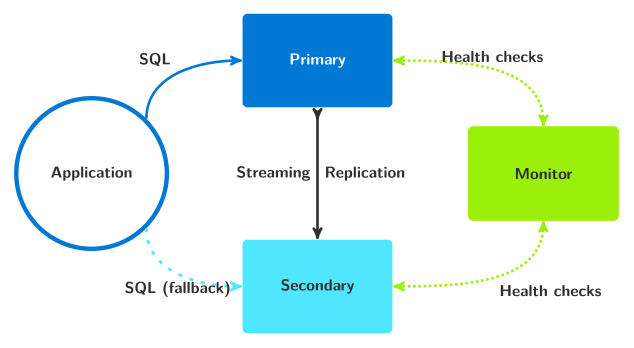
\includegraphics[width=0.75\linewidth]{source/implementation/evaluation/postgresql_ha_solutions/pg_auto_failover/pg_auto-failover_arch-single-standby}
        \caption{pg\_auto\_failover-Architektur - Single Standby}
        \label{fig:pg_auto-failover_arch-single-standby}
    \end{figure}
    Aber wie die Grafik zeigt, können auch Multi-Nodes können eingebunden werden\cite{4ZKBDG57}:
    \begin{figure}[H]
        \centering
        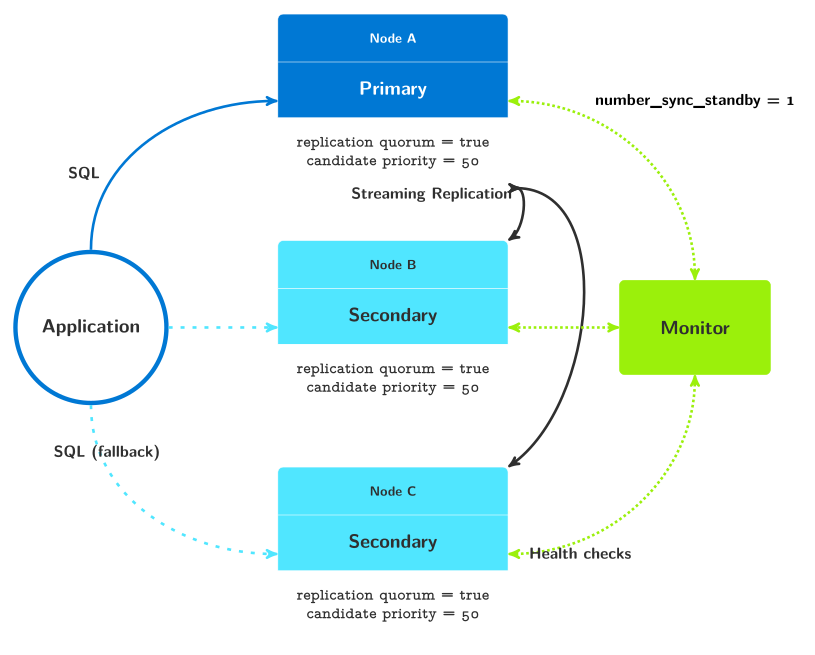
\includegraphics[width=0.75\linewidth]{source/implementation/evaluation/postgresql_ha_solutions/pg_auto_failover/pg_auto-failover_arch-multi-standby}
        \caption{pg\_auto\_failover-Architektur - Multi-Node Standby}
        \label{fig:pg_auto-failover_arch-multi-standby}
    \end{figure}

    pg\_auto\_failover kann Citus einbinden.
    Allerdings bleibt die Architektur im Kern immer monolithisch.\\
    ie nachfolgende Grafik zeigt die Architektur mit Citus\cite{3FVHLIFE}:
    \begin{figure}[H]
        \centering
        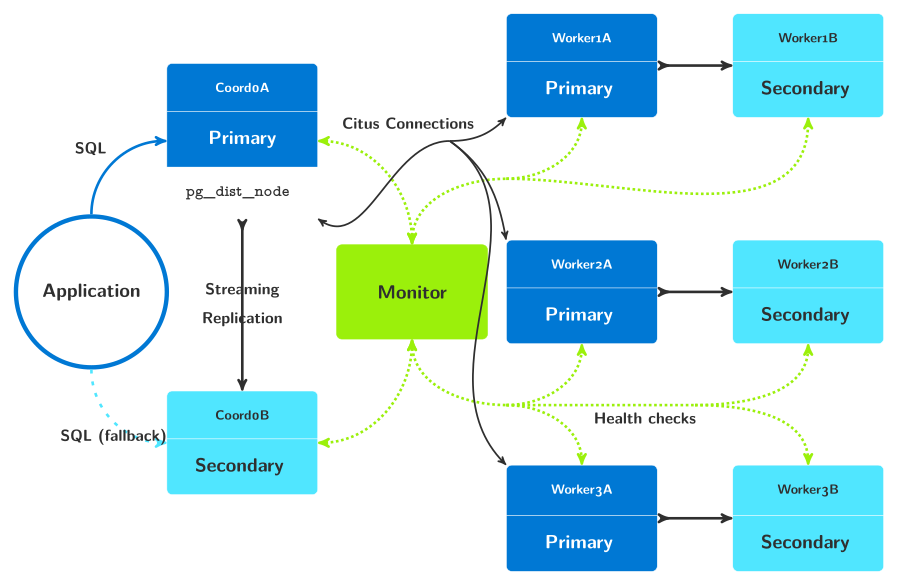
\includegraphics[width=0.75\linewidth]{source/implementation/evaluation/postgresql_ha_solutions/pg_auto_failover/pg_auto-failover_arch-citus}
        \caption{pg\_auto\_failover-Architektur - Citus}
        \label{fig:pg_auto-failover_arch-citus}
    \end{figure}
\end{flushleft}
\begin{flushleft}
    \paragraph{Synergien und Mehrwert}
    pg\_auto\_failover bietet eine Docker-Compose-Integration.\\
    Allerdings ist keine Kubernetes-Integration dokumentiert.
\end{flushleft}
\begin{flushleft}
    Damit bietet pg\_auto\_failover keine Möglichkeit\\
    Synergien zwischen monolithischer Architektur und einer Cloud-Native-Umsetzung auf Kubernetes.\\
    Entsprechend ist kein Mehrwert vorhanden.
\end{flushleft}